\section{Introduction}
In 1965, the statistician Stanley Warner noticed that for sensitive questions, survey participation was hampered by the unwillingness of participants to confide in an interviewer \cite{warner1965randomized}.
Consider an auditor exploring the prevalence of bribery in a government office through a survey question: \emph{Yes or No, have you accepted bribe in the last year?}. 
Even with guarantees of anonymity, employees may be reluctant to provide truthful responses.
For such scenarios, Warner proposed the \emph{Randomized Response} model: (1) a participant flips a coin before the interview, (2) if heads, he answers truthfully, and (2) if tails, he selects Yes or No uniformly at random.
Warner showed that such a model provides participants with plausible deniability about their response, yet still allows for rigorous statistical estimation and hypothesis testing.

Since 1965, there have been number of proposals to guarantee privacy while preserving some utility like homeomorphic encryption, value aggregation, and selective censorship \cite{sweeney2002achieving, machanavajjhala2007diversity, li2007t}.
While the aforementioned techniques allow for query answering on private data, they obscure the actual values.
However, raw data rarely starts off in a useful form, and an analyst has to perform a number of preprocessing steps including extraction and resolving inconsistencies prior to query answering--all of which be definition require access to the actual record attribute values.
On the other hand, consider a generalization of Warner's model, where for discrete-valued attributes with probability $p$ replace the value uniformly at random with another value in the domain.   
While any given record can be incorrect, for a large enough dataset, all of the domain values are likely to appear in the the randomized result.
It follows that some types of data cleaning operations, e.g., a find-and-replace, may be possible even on randomized relations (Figure \ref{example}).

However, the challenge is to like Warner's model to meaningful notion of data privacy.
$\epsilon$-differential privacy model~\cite{dwork2011differential} quantifies the privacy of randomized mechanisms.
This is a probabilistic definition of privacy, where $\epsilon$ represents the increase in probability of correctly identifying an individual's response given all other records in a database.
It can be shown that Warner's model is in fact $\epsilon$ differentially private, where $\epsilon$ is inversely related to the randomization probability $p$.
One of the key challenges is selecting meaningful parameter values for the task at hand, i.e., what is the practical difference between $\epsilon = \ln 3$ compared to $\epsilon = \ln 5$~\cite{DBLP:conf/sigmod/YangZMWX12}.

\begin{figure}[t]
\centering
 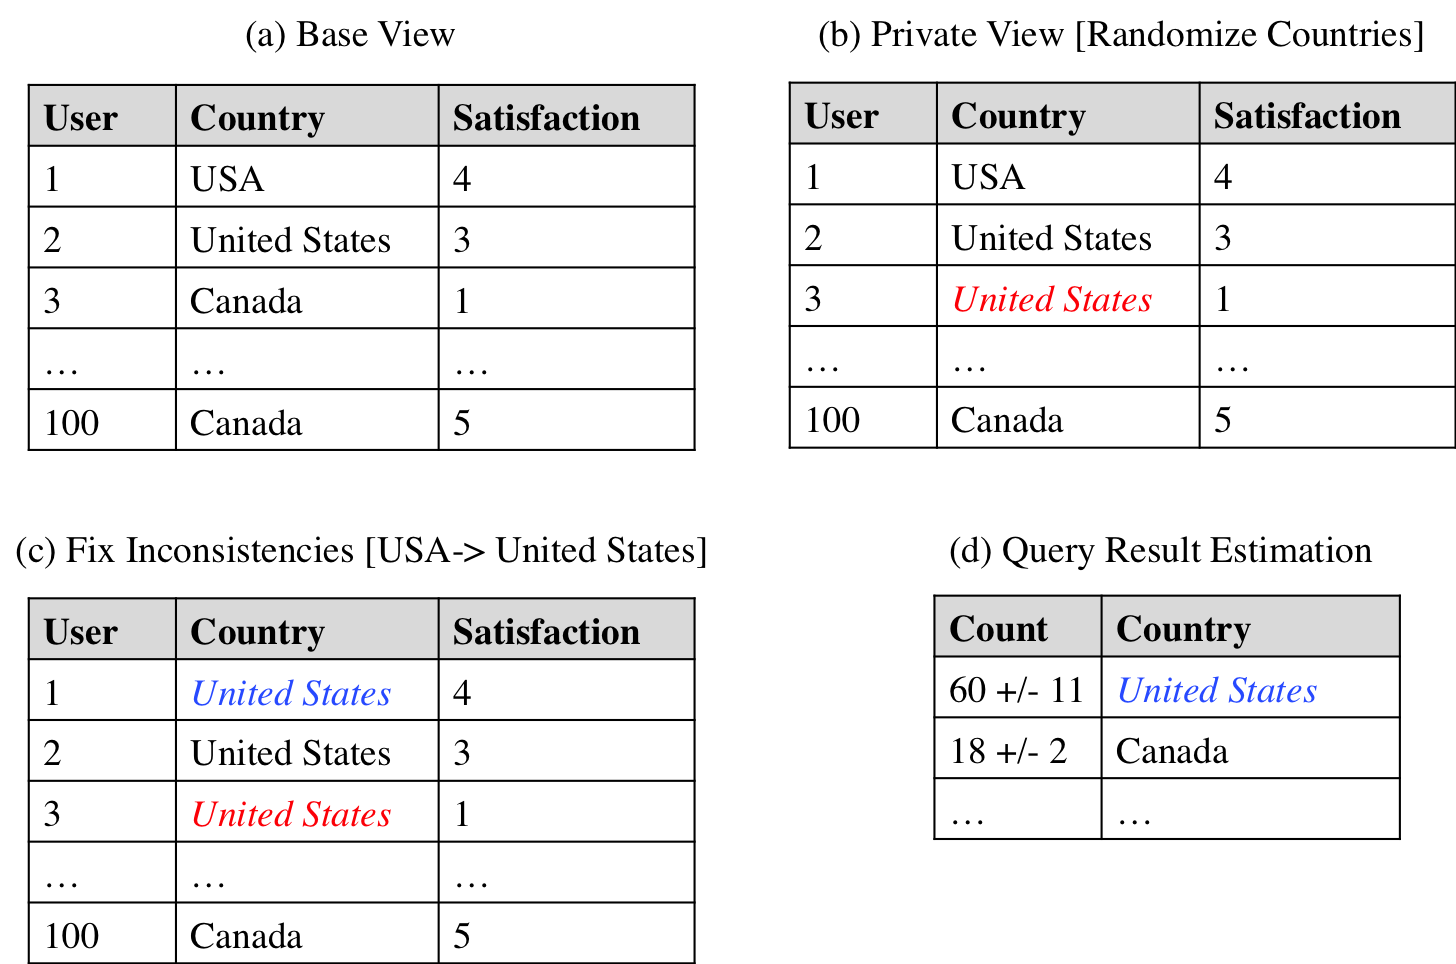
\includegraphics[width=\columnwidth]{figs/example.png}
 \caption{\sys allows users to perform a limited set of cleaning operations on private views of data. Differential privacy preserves attribute domains, and thus, inconsistencies can be identified in even provably private views.\label{example}}\vspace{-2em}
\end{figure}

In this paper, we present \sys a framework for data cleaning and approximate query processing on differentially private relations.
We assume that there is a trusted curator of a database $D$, and an untrusted analyst who wishes to analyze a view of this database $V$ which consists of numerical (integer or real valued) attributes and possible dirty discrete valued attributes.
We apply a generalized version of Warner's randomized response technique called, Generalized Randomized Response (GRR), to the view $V$.
This view is provably private for any desired level of privacy $\epsilon$.
Analysts can apply a restricted set of deterministic data cleaning operations to clean the dirty discrete attributes.
Then, we provide an estimation framework to estimate the result of \sumfunc, \countfunc, and \avgfunc queries on the cleaned private relation.
The system is self-tuning and can select a level of privacy to ensure that any dirtiness in the discrete attributes can be detected with probability of at least $1-\alpha$ or that all subsequent aggregate queries are guaranteed to be within $\delta\%$ accuracy with high probability.

There are a number of technical contributions in this paper.
First, we formalize the class of data cleaning operations that can be supported on a GRR view, and we model the effects of data cleaning as a bi-partite graph mapping dirty values to cleaned values.
We can use this graph to estimate false positive values included in aggregate queries with predicates. 
Next, we analyze the system statistically both in the finite-sample case and in the asymptotic case to understand the tradeoff between privacy, cleanability, and query accuracy.
Finally, we show how this analysis can be inverted to select maximal privacy levels given some constraint on query accuracy or cleanability.















